\documentclass[spanish]{beamer}
\usepackage[ansinew]{inputenc} % Acepta caracteres en castellano
\usepackage[spanish]{babel}    % silabea palabras castellanas
\usepackage{amsmath}
\usepackage{mathtools,cancel} % cancela con una flecha \cancelto{0}{XXXX}
\renewcommand{\CancelColor}{\color{red}} %change cancel color to red
\usepackage{amsfonts}
\usepackage{amssymb}
\usepackage{dsfont}
\usepackage{graphicx}
\usepackage{geometry}
\usetheme{Madrid}
\usecolortheme{beaver}
\usepackage{textpos}
% Logo  en el comienzo 
\addtobeamertemplate{frametitle}{}{%
\begin{textblock*}{100mm}(.85\textwidth,-1cm)
{\includegraphics[height=0.4in, keepaspectratio=true]{/Users/luisnunez/Dropbox/MisDocumentos/UIS/UISImagenInstitucional/UISLOGO.png}}
\end{textblock*}}

\begin{document}

\title{\textbf{Vector Laplace-Runge-Lenz} }
\author[L.A. N��ez]{\textbf{Luis A. N��ez}}  
\institute[UIS]{\textit{Escuela de F�sica, Facultad de Ciencias, } \\
\textit{Universidad Industrial de Santander, Santander, Colombia } \\
{\includegraphics[height=0.4in, keepaspectratio=true]{/Users/luisnunez/Dropbox/MisDocumentos/UIS/UISImagenInstitucional/UISLOGO.png}}
}
\date{\today}
\maketitle


\begin{frame}
\frametitle{Agenda}
  \tableofcontents
\end{frame}


%%%%% Diapo 1
\section{El problema de Kepler y el vector $\mathbf{A}$, Laplace-Runge-Lenz }
\frame{
  \frametitle{El vector $\mathbf{A}$}
   \begin{itemize}  
  	\item<1-> La trayectoria del problema de Kepler con el potencial central $V(r)=-k / r$ y la fuerza gravitacional $\mathbf{f}(r)=f(r) \hat{\mathbf{r}}$, con $f(r)=-k / r^2$, es una secci�n c�nica, $\frac{q}{r}=1+e \cos \theta$, donde $q=L^2 / \mu k$, y $e=\sqrt{1+\frac{2 E L^2}{\mu k^2}}$.
	\item<2-> Podemos definir $\mathbf{r} \cdot \mathbf{A}= r A \cos \theta = L^2-\mu k r$, con $A \equiv \mu k e =$ cte.
	\item<3-> $\mathbf{A}$ es un vector de magnitud es constante y direcci�n debe estar en la direcci�n del perihelio. Si la direcci�n est� en el eje $x$,  $\mathbf{A}=\mu k e \hat{\mathbf{i}}$.
	\begin{figure}[t]
		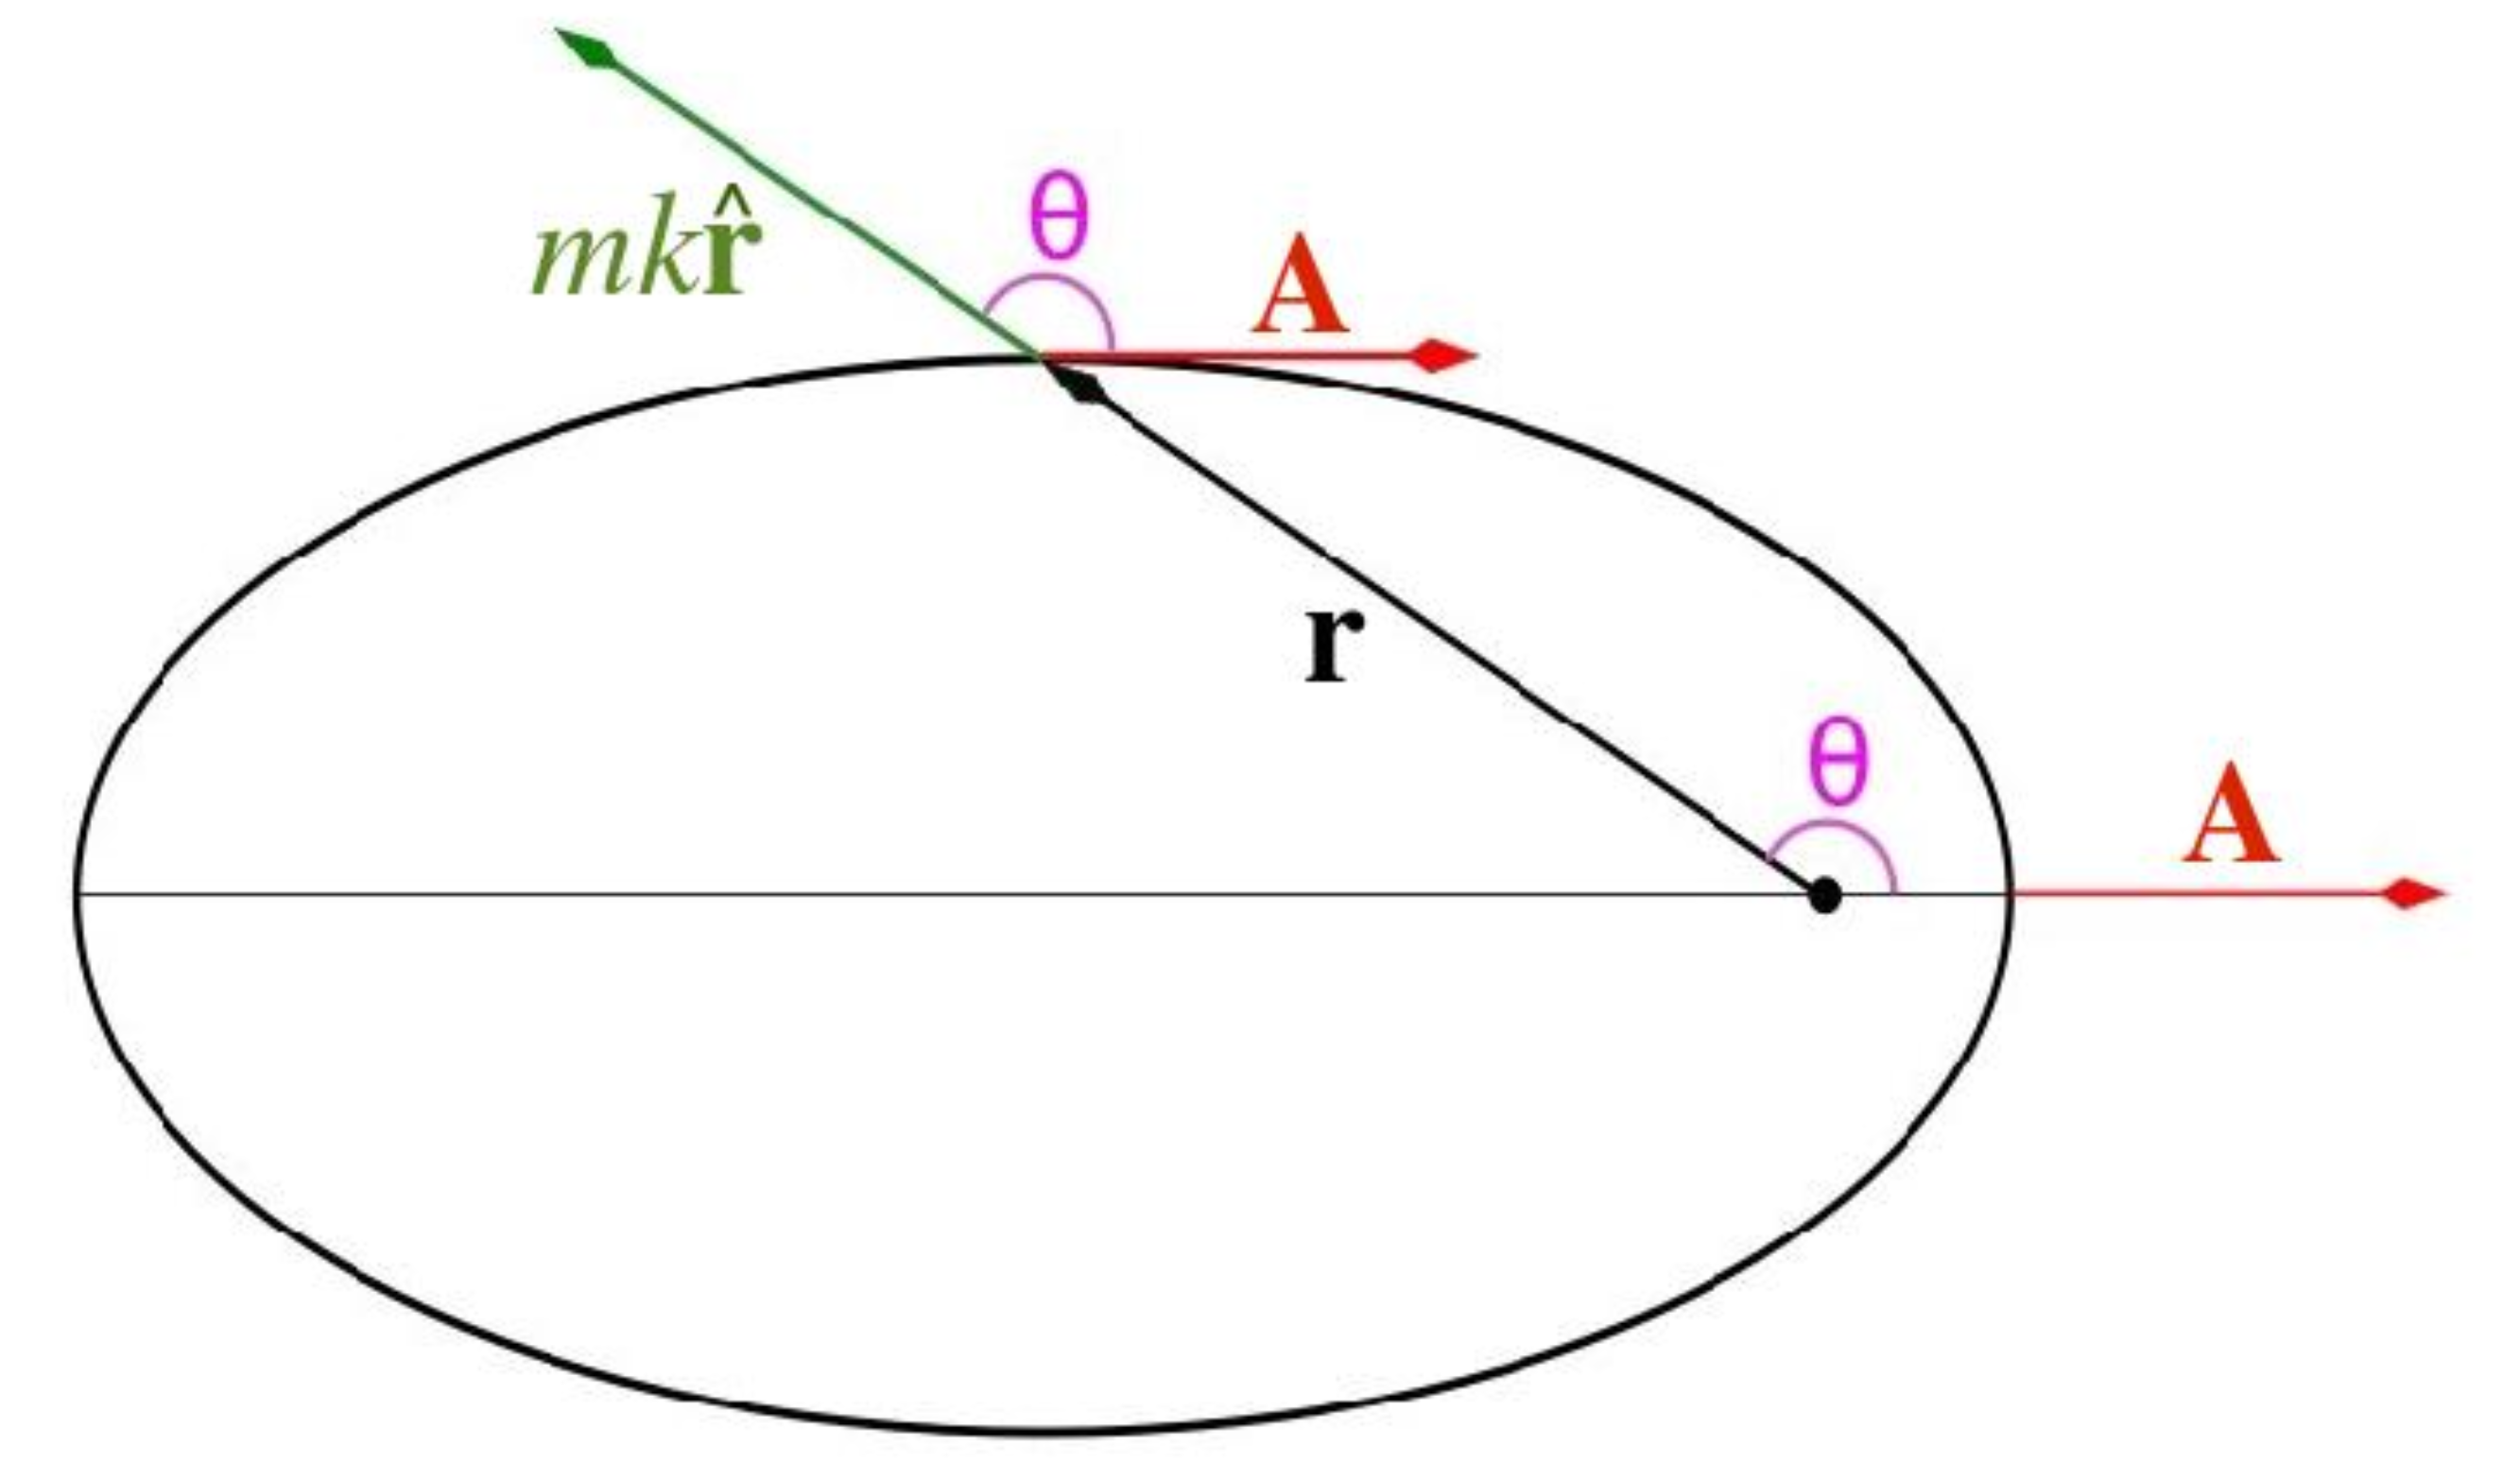
\includegraphics[width=1.8in]{Figuras/VectorA.png}
   	\end{figure}
	\item<4-> Como $L^2=\mathbf{L} \cdot \mathbf{L}=\mathbf{L} \cdot(\mathbf{r} \times \mathbf{p})=\mathbf{r} \cdot(\mathbf{p} \times \mathbf{L}) \Rightarrow \mathbf{r} \cdot \mathbf{A}=\mathbf{r} \cdot[(\mathbf{p} \times \mathbf{L})-\mu k \hat{\mathbf{r}}]$
	\item<5-> Donde $\mathbf{A} \equiv \mathbf{p} \times \mathbf{L} -\mu k \hat{\mathbf{r}}$ y tambi�n $\mathbf{A} \cdot \mathbf{L}=0$
	 
    \end{itemize}
}
%%%%% Diapo 2
\section{El vector $\mathbf{A}$ como cantidad conservada}
\frame{
  \frametitle{$\mathbf{A}$ es cantidad conservada}
   \begin{itemize}  
  	\item<1-> Consideremos $\frac{d \mathbf{A}}{d t}=\frac{d}{d t}(\mathbf{p} \times \mathbf{L})-\mu k \frac{d \hat{\mathbf{r}}}{d t}$
	\item<2-> El primer t�rmino $\frac{d}{d t}(\mathbf{p} \times \mathbf{L})=\frac{d \mathbf{p}}{d t} \times \mathbf{L}+\mathbf{p} \times \cancelto{0}{\frac{d \mathbf{L}}{d t}} =\frac{d \mathbf{p}}{d t} \times(\mathbf{r} \times \mu \mathbf{v})$
	\item<3-> Por otro lado, $\frac{d \mathbf{p}}{d t}=\mathbf{f}(r)=f(r) \hat{\mathbf{r}}=f(r) \frac{\mathbf{r}}{r}$ 
	\item<4-> Entonces $\frac{d}{d t}(\mathbf{p} \times \mathbf{L})=\mu \frac{f(r)}{r}\left[\mathbf{r} \times\left(\mathbf{r} \times \frac{d \mathbf{r}}{d t}\right)\right] = \mu \frac{f(r)}{r}\left[\mathbf{r}\left(\mathbf{r} \cdot \frac{d \mathbf{r}}{d t}\right)-r^2 \frac{d \mathbf{r}}{d t}\right] $ \\ ya que $\mathbf{a} \times(\mathbf{b} \times \mathbf{c})=\mathbf{b}(\mathbf{a} \cdot \mathbf{c})-\mathbf{c}(\mathbf{a} \cdot \mathbf{b})$
	\item<5-> Como $\frac{d}{d t}(\mathbf{r} \cdot \mathbf{r})=2 \mathbf{r} \cdot \frac{d \mathbf{r}}{d t}=\frac{d}{d t}\left(r^2\right)=2 r \frac{d r}{d t}$ 
	\item<6-> Tendremos $\frac{d}{d t}(\mathbf{p} \times \mathbf{L})=\mu f(r)\left[\mathbf{r} \frac{d r}{d t}-r \frac{d \mathbf{r}}{d t}\right]$
	\item<7-> Adem�s $\frac{d}{d t}\left(\frac{\mathbf{r}}{r}\right)  =\frac{d \mathbf{r}}{d t} \frac{1}{r}-\frac{\mathbf{r}}{r^2} \frac{d r}{d t} \Rightarrow \quad-r^2 \frac{d}{d t}\left(\frac{\mathbf{r}}{r}\right)  =\mathbf{r} \frac{d r}{d t}-r \frac{d \mathbf{r}}{d t}$
	\item<8-> Con lo cual $\frac{d}{d t}(\mathbf{p} \times \mathbf{L})=-\mu f(r) r^2 \frac{d}{d t}\left(\frac{\mathbf{r}}{r}\right) = \mu k \frac{d}{d t}\left(\frac{\mathbf{r}}{r}\right)=\mu k \frac{d \hat{\mathbf{r}}}{d t}$ para $f(r)=-k / r^2$
	\item<9-> y finalmente $\frac{d \mathbf{A}}{d t}=0 \Rightarrow \mathbf{A} \equiv \mathbf{p} \times \mathbf{L} -\mu k \hat{\mathbf{r}} =$cte

\end{itemize}
}

%%%%% Diapo 2
\section{Problema Kepler superintegrable}
\frame{
\frametitle{Kepler superintegrable}
\begin{itemize}  
	\item<1-> La magnitud del vector \textbf{A} para la fuerza gravitacional se expresa en t�rminos de $L$ y $E$ como $A^2=(\mu k e)^2=\mu^2 k^2+2 \mu E L^2=$ cte
	\item<2-> La direcci�n de $\mathbf{A}$, correspondiente a la direcci�n del perihelio, provee una nueva cantidad conservada en el problema de Kepler.
	\begin{figure}[t]
		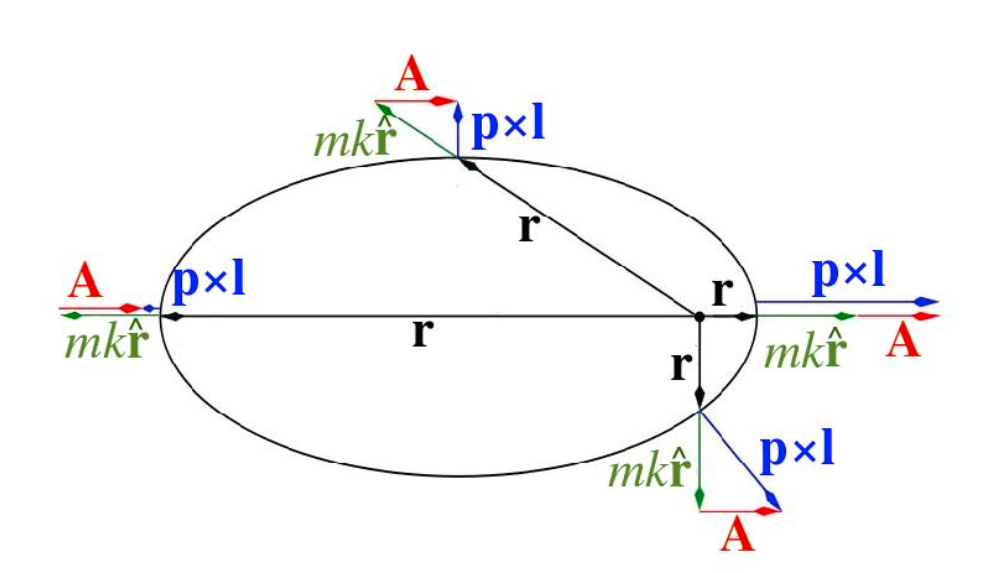
\includegraphics[width=1.5in]{Figuras/DirA.png}
   	\end{figure}
	\item<3-> El sistema de dos cuerpos sujetos a la fuerza gravitacional que var�a como el inverso del cuadrado de la distancia constituye un sistema superintegrable. La constancia de la direcci�n $\hat{\mathbf{A}}$ implica que una �rbita en el potencial $V(r)=-k / r$ no presenta precesi�n.
	\item<4-> Existen seis grados de libertad (tres para cada part�cula) y siete cantidades conservadas: las tres componentes de la velocidad del centro de masa $\mathbf{v}_{c m}$, la direcci�n del momento angular $\mathbf{L}$, su magnitud $L$, la energ�a $E$ y la direcci�n del vector de Laplace-Runge-Lenz $\hat{\mathbf{A}}$

\end{itemize}
}
%%%%% Diapo 2
\section{Secci�n}
\frame{
  \frametitle{T�tulo transparencia}
   	\begin{itemize}  
  \item<1-> 
    \end{itemize}
}
%%%%% Diapo 2
\section{Secci�n}
\frame{
  \frametitle{T�tulo transparencia}
   	\begin{itemize}  
  \item<1-> 
    \end{itemize}
}
%%%%% Diapo 2
\section{Secci�n}
\frame{
  \frametitle{T�tulo transparencia}
   	\begin{itemize}  
  \item<1-> 
    \end{itemize}
}
  
\end{document}
